\section{Durchführung}
\label{sec:Durchführung}
Der Aufbau des Versuches besteht aus einer optischen Bank, verschiedenen Linsen, einem Schirm und einer Halogenlampe. Als Probegegenstand wird ein rechtwinklig überlappendes Kreuz aus zwei gleichlangen Pfeilen verwendet, welche als negativ aus einer Lichtundurchlässigen Platte geschnitten worden sind. Dieser Probegegenstand wird der einfachaltshalber im folgenden als \glqq Kreuz\grqq{} bezeichnet.

\subsection{Bestimmung der Brennweite einer Linse über die Gegenstands- und Bildweite} % (fold)
\label{sub:Bestimmung der Brennweite einer Linse}
Die Halogenlampe, das Kreuz, eine Linse mit bekannter Brennweite und der Bildschrim werden in dieser Reihenfolge auf der Höhe des Lichtstrahls der Lampe ausgerichtet. Bei fester Gegenstandsweite wird die Entfernung des Bildschirms so lange verändert, bis ein scharfes Bild auf dem Bildschirm zu sehen ist. In dem Fall und im weiteren Versuch wird von einem scharfen Bild die Rede sein, wenn ein möglichst unverschmierter Punkt auf dem Bildschirm zu sehen ist. Die Gegegenstandsweite und die Bildweite werden notiert.
Dieser Vorgang wird für weitere zehn Gegegenstandsweiten wiederholt. 


Daraufhin wird das gleiche Verfahren für eine zweite Linse durchgeführt.


\subsection{Methode von Bessel} % (fold)
\label{sub:Methode von Bessel}
Erneut gilt es, die Brennweite einer Linse zu bestimmen. Diesmal wird dafür die Methode von Bessel verwendet. Die optische Bank bleibt unverändert im Aufbau. Bei dieser Methode bleiben Bildschirm und Gegenstand fest an einer Stelle. Dazwischen wird eine Linse solange verschoben, bis ein scharfes Bild auf dem Schirm entsteht. Da es sich um eine symmetrische Linsenstellung handelt, tritt ein scharfes Bild an zwei Linsenpositionen auf. Gegegenstands- und Bildweite werden jeweils notiert. Dieser Vorgang wird wieder für zehn weitere Entfernungen zwischen Kreuz und Schirm durchgeführt.

Über 
\begin{equation}
    f=\frac{e^2-d^2}{4e}
    \label{eqn:besself}
\end{equation}
lässt sich die Brennweite der verwendeten Linse bestimmen. Dabei beschreibt $e$ den Abstand zwischen Kreuz und Schirm und $d$ den Abstand der beiden Linsenpositionen, an denen ein scharfes Bild auf dem Schirm entsteht.
Der Abbildung \ref{fig:Bessel} ist zu entnehmen, dass sich der Abstand zwischen Kreuz und Schirm über
\begin{equation}
    e=g_1+b_1=g_2+b_2
\end{equation}
und der Abstand zwischen den Linsenpositionen über
\begin{equation}
    d=g_1-b_1=g_2-b_2
\end{equation}
berechnen lässt.


\begin{figure}
    \centering
    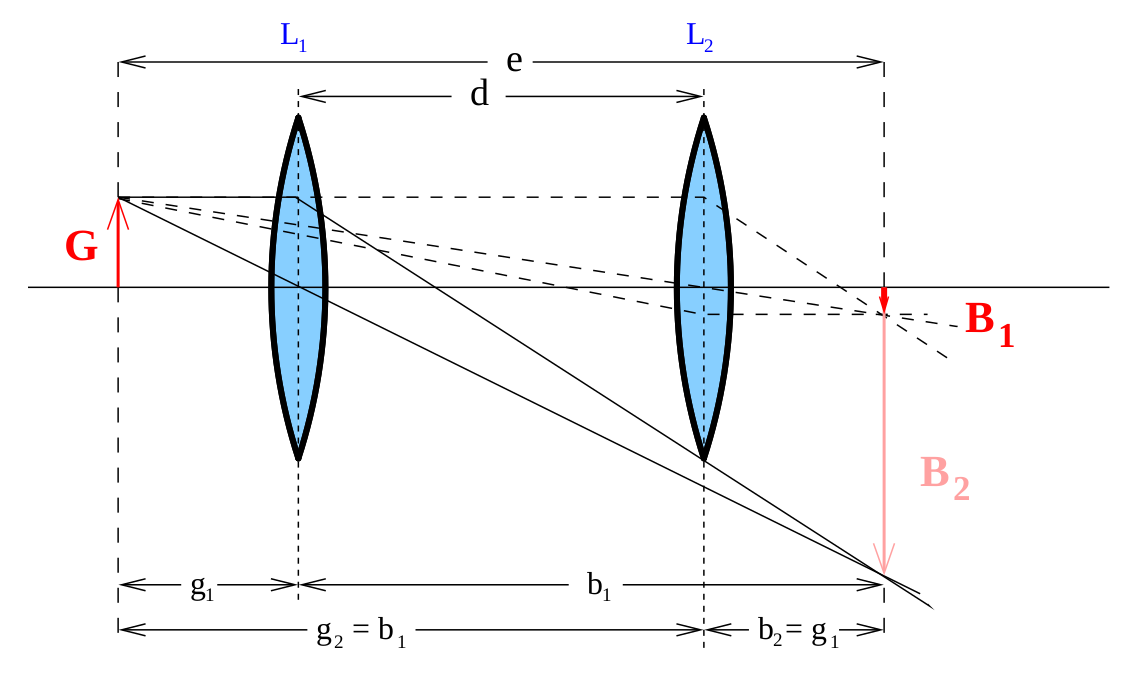
\includegraphics[width=\textwidth]{data/Bessel.png}
    \caption{Darstellung der beiden Linsenpositionen bei der Bessel-Methode.}
    \label{fig:Bessel}
\end{figure}


Die Bessel-Methode wird ein weiteres mal unter dem gleichen Aufbau durchgeführt. Dabei wird diesmal für jeweils fünf Messvorgänge ein roter oder blauer Filter in den Mündungslichtstrahl der Lampe gehalten. Dies hat die Untersuchung der chromatischen Abberration zum Zweck.



% subsection Methode von Bessel (end)
% subsection Bestimmung der Brennweite einer Linse (end)
%Was wurde gemessen bzw. welche Größen wurden variiert?